\documentclass[12pt]{article}
\usepackage[utf8]{inputenc}
\usepackage{fullpage}
\usepackage{graphicx}
\usepackage{enumitem}
\usepackage{hanging}
\usepackage{lipsum}
\usepackage{svg}
\usepackage{amsmath}
\usepackage{xcolor}
\usepackage{soul}
\usepackage{color}
\usepackage[usenames,dvipsnames]{xcolor}
\usepackage{lastpage} % Required to determine the last page number for the footer
\usepackage{graphicx} % Required to insert images
\setlength\parindent{0pt} % Removes all indentation from paragraphs
\usepackage[most]{tcolorbox} % Required for boxes that split across pages
\usepackage{booktabs} % Required for better horizontal rules in tables
\usepackage{listings} % Required for insertion of code
\usepackage{etoolbox} % Required for if statements
\usepackage{geometry} % Required for adjusting page dimensions and margins
\usepackage{wrapfig}
\usepackage{algorithm}
\usepackage{algorithmic}
\usepackage{hyperref}
\usepackage{pdflscape}

\newcommand{\hlc}[2][yellow]{ {\sethlcolor{#1} \hl{#2}} }

\geometry{
	paper=a4paper, % Change to letterpaper for US letter
	top=3cm, % Top margin
	bottom=3cm, % Bottom margin
	left=2.5cm, % Left margin
	right=2.5cm, % Right margin
	headheight=14pt, % Header height
	footskip=1.4cm, % Space from the bottom margin to the baseline of the footer
	headsep=1.2cm, % Space from the top margin to the baseline of the header
	%showframe, % Uncomment to show how the type block is set on the page
}
\pagestyle{fancy} % Enable custom headers and footers



\title{IVR CW}
\author{Yannik Nelson}

\begin{document}
\maketitle
\tableofcontents \newpage

\section{Robot Vision}
\subsection{Joint State Estimation}
The first step of finding the joint angles involves finding the position of the joint blobs. To do this, i threshold each image to isolate each joint, I then find the moments in the thresholded image (should only have one for each joint) and return the center of that moment (if there is no moment found then I return the center of the last moment found for the image plane being viewed and the colour being thresholded).
\newline \newline
This then leaves me with in-image coordinates for each joint from each camera, to find the 3D world coordinates relative to the base joint (yellow joint) I first find the pixel to meter scales for each image by taking the distance from the blue joint to the yellow joint and dividing 2.5 by that value. To find the X coordinate I subtract the yellow joint position in the zx image from the position of the desired joint in the zx image, take the image x coordinate of that and time it by the scale for that image. I do the same thing to find the Y coordinate but using the zy image positions and scale instead. Finally to find the Z coordinate perform the same operation for both images taking the image Y coordinate instead and then take the average of the values from the two images (this attempts to deal with perspective but doesn't do very well).
\newline \newline
To then find the angle of each joint i attempted multiple methods:
\begin{itemize}
    \item Joint 2
    \begin{itemize}
        \item I started by trying to project the vector corresponding the link 3 (the link between the blue and green joints) only the zy plane and then taking the angle between that the [0,0,1] vector (straight up).
        \item I then used the kinematic equation describing the position of the green joint which gave the y value = $-3.5s\left(\theta_{2}\right)c\left(\theta_{3}\right)$, z value = $3.5c\left(\theta_{2}\right)c\left(\theta_{3}\right) + 2.5$. Using these $\frac{y}{z} = -\tan(\theta_{2})$. I attempted using that equation rearranged to get $\theta_{2}$, this didn't work.
        \item I finally took the angle of the vector from where the blue joint should be [0,0,2.5] and the measured position of the blue joint(the blue joint moved as it rotated), this produced the best results.
    \end{itemize}
    \item Joint 3
    \begin{itemize}
        \item I take the angle between the link 3 vector and the zy plane, this produces almost exact results.
    \end{itemize}
    \item Joint 4
    \begin{itemize}
        \item I take the angle between the link 3 vector and the link 4 vector and then invert the sign based on the relative positions of the blue and green joints and the zx plane. The angle absolute value performs reasonably well, the sign does not, I did not have time to improve this performance.
    \end{itemize}
\end{itemize}
\newline \nelwine
Here is the plot of my Joint State Estimations against their expected values:\newline
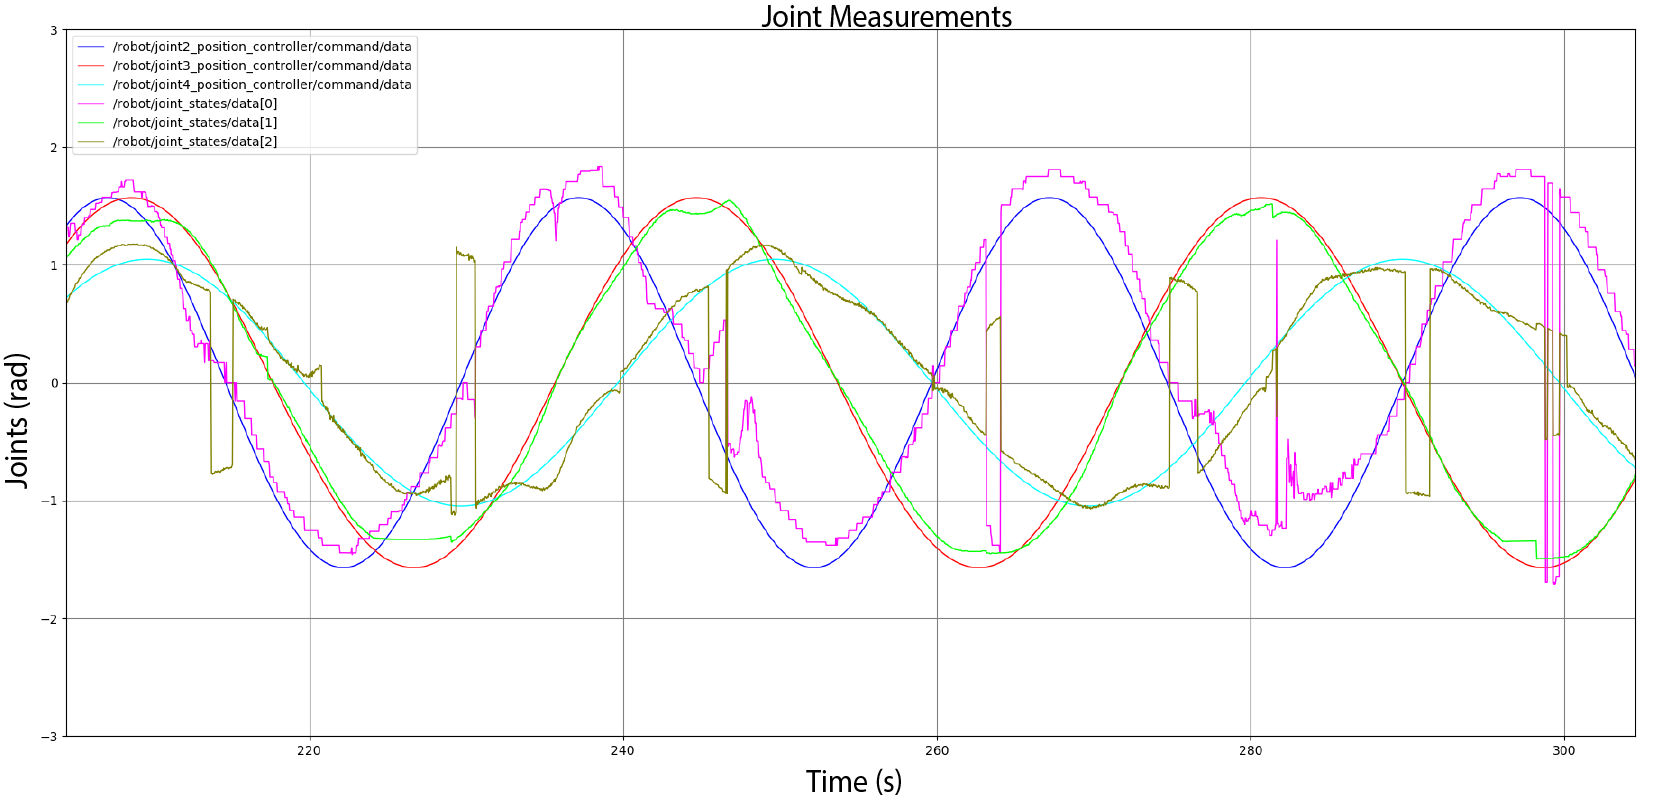
\includegraphics[width=\textwidth]{best angle tracking.png}
Here you can see that the accuracy of the $\theta_3$ (measured = green, expected = red) tracking is almost exact save for the times the green joint goes out of view of one of the cameras which produces a flat part in the green plot.\newline\newline
The $\theta_2$ (measured = pink, expected = blue) tracking performs reasonbly well but becomes less accurate and more noisy as $\theta_3$ gets far from 0, this is due to the perspective causing the Z of the green joint to appear lower than the blue joint, which shouldn't be possible.\newline\newline
The $\theta_4$ tracking performs reasonably well with the exception of incorrectly jumping sign when $\theta_2$ is near zero, or when the blue joint is crossing the zx plane, this is because the conditions used to determine the sign of the angle work best when the blue joint is far from the zx plane but become too simple as it gets close, I did not have time to come up with better checks.\newpage
\subsection{Target Detection}
Here is the plot of the detected X Y and Z positions of the target plotted against the real values:\newline
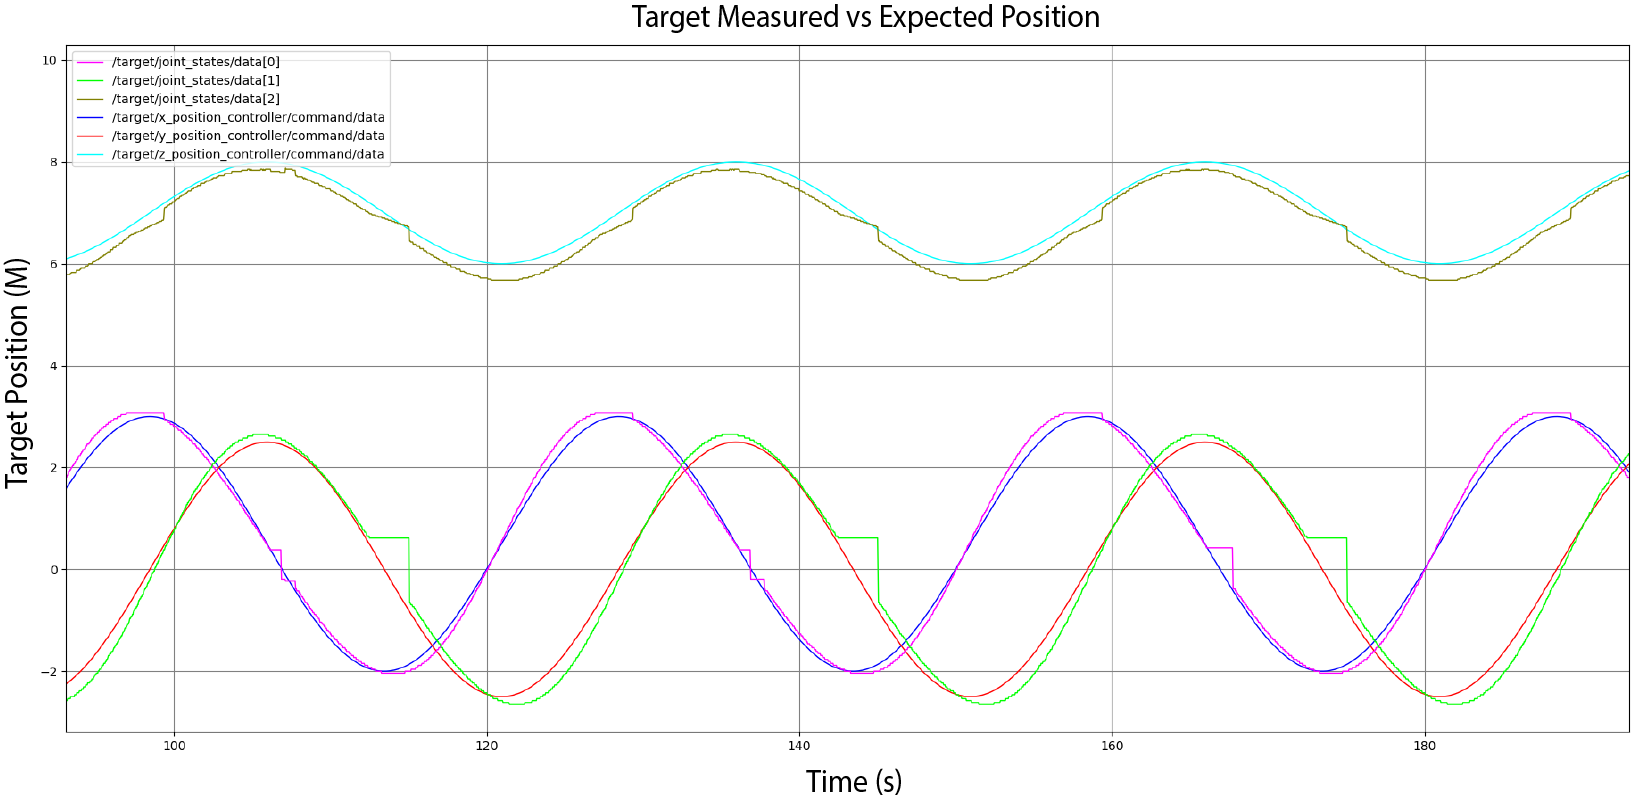
\includegraphics[width=\textwidth]{target_tracker.png}
My algorithm works by taking in templates for the target and the box for each view and finding the contours for each at initialisation.
My algorithm then thresholds the images received from each camera, uses the cv2.findContours() function to find the contours and the cv2.matchShape() to check each contour against both the box and the target template contours, the result from these comparisons are checked and if the match to the target is greater than the match to the box then the moment for that contour is found, the center is extracted from that moment and that center is returned. If the algorithm doesn't isn't more sure either of the contours is the target then it will return the last saved position of the target in the respective view. I then find the x y z values from the position in the image as before. \newline
In the plot you can see flat parts and jumps in plots of the measured values. The spikes occur due to instances where partial obstruction of the wall or target causes the shape matching to confuse the target and the orange box. The Flat parts occur due to the obstruction of the target as well, except in these cases the shape matching 'catches' that the box is not the target and so doesn't change the measured position of the target until it's visible again.
\newpage
\section{Robot Control}
\subsection{Robot Kinematics}
D-H representation:\newline
\begin{center}
    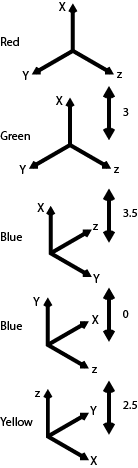
\includegraphics[]{D-H.png}
\end{center}\newline
D-H Table:
\begin{center}
    \begin{tabular}{c|c c c c}
         & \alpha & a & d & \theta \\ \hline
        1 & $\frac{\pi}{2}$ & 0 & 2.5 & $\theta_1 + \frac{\pi}{2}$\\
        2 & $\frac{\pi}{2}$&  0 & 0 & $\theta_2 + \frac{\pi}{2}$\\
        3 & $-\frac{\pi}{2}$ & 3.5 & 0 & \theta_3 \\
        4 & 0 & 3 & 0 & \theta_4\\
    \end{tabular}
\end{center}\newline
\begin{center}
    A_1^0 = $\left[\begin{matrix}c{\left(\theta_{1} + \frac{\pi}{2}\right)} & - s{\left(\theta_{1} + \frac{\pi}{2}\right)} & 0 & 0\\s{\left(\theta_{1} + \frac{\pi}{2}\right)} & c{\left(\theta_{1} + \frac{\pi}{2}\right)} & 0 & 0\\0 & 0 & 1 & 0\\0 & 0 & 0 & 1\end{matrix}\right]$$\left[\begin{matrix}1 & 0 & 0 & 0\\0 & 1 & 0 & 0\\0 & 0 & 1 & 2.5\\0 & 0 & 0 & 1\end{matrix}\right]$$\left[\begin{matrix}1 & 0 & 0 & 0\\0 & 1 & 0 & 0\\0 & 0 & 1 & 0\\0 & 0 & 0 & 1\end{matrix}\right]$$\left[\begin{matrix}1 & 0 & 0 & 0\\0 & c{\left(\frac{\pi}{2} \right)} & - s{\left(\frac{\pi}{2} \right)} & 0\\0 & s{\left(\frac{\pi}{2} \right)} & c{\left(\frac{\pi}{2} \right)} & 0\\0 & 0 & 0 & 1\end{matrix}\right]$\newline
    = $\left[\begin{matrix}- s{\left(\theta_{1} \right)} & 0 & c{\left(\theta_{1} \right)} & 0\\c{\left(\theta_{1} \right)} & 0 & s{\left(\theta_{1} \right)} & 0\\0 & 1 & 0 & 2.5\\0 & 0 & 0 & 1\end{matrix}\right]$\newline\newline
    
    A_2^1 = $\left[\begin{matrix}c{\left(\theta_{2} + \frac{\pi}{2}\right)} & - s{\left(\theta_{2} + \frac{\pi}{2}\right)} & 0 & 0\\s{\left(\theta_{2} + \frac{\pi}{2}\right)} & c{\left(\theta_{2} + \frac{\pi}{2}\right)} & 0 & 0\\0 & 0 & 1 & 0\\0 & 0 & 0 & 1\end{matrix}\right]$$\left[\begin{matrix}1 & 0 & 0 & 0\\0 & 1 & 0 & 0\\0 & 0 & 1 & 0\\0 & 0 & 0 & 1\end{matrix}\right]$$\left[\begin{matrix}1 & 0 & 0 & 0\\0 & 1 & 0 & 0\\0 & 0 & 1 & 0\\0 & 0 & 0 & 1\end{matrix}\right]$$\left[\begin{matrix}1 & 0 & 0 & 0\\0 & c{\left(\frac{\pi}{2} \right)} & - s{\left(\frac{\pi}{2} \right)} & 0\\0 & s{\left(\frac{\pi}{2} \right)} & c{\left(\frac{\pi}{2} \right)} & 0\\0 & 0 & 0 & 1\end{matrix}\right]$\newline
    $\left[\begin{matrix}- s{\left(\theta_{2} \right)} & 0 & c{\left(\theta_{2} \right)} & 0\\c{\left(\theta_{2} \right)} & 0 & s{\left(\theta_{2} \right)} & 0\\0 & 1 & 0 & 0\\0 & 0 & 0 & 1\end{matrix}\right]$\newline\newline
    
    A_3^2 = $\left[\begin{matrix}c{\left(\theta_{3}\right)} & - s{\left(\theta_{3} \right)} & 0 & 0\\s{\left(\theta_{3} \right)} & c{\left(\theta_{3} \right)} & 0 & 0\\0 & 0 & 1 & 0\\0 & 0 & 0 & 1\end{matrix}\right]$$\left[\begin{matrix}1 & 0 & 0 & 0\\0 & 1 & 0 & 0\\0 & 0 & 1 & 0\\0 & 0 & 0 & 1\end{matrix}\right]$$\left[\begin{matrix}1 & 0 & 0 & 3.5\\0 & 1 & 0 & 0\\0 & 0 & 1 & 0\\0 & 0 & 0 & 1\end{matrix}\right]$$\left[\begin{matrix}1 & 0 & 0 & 0\\0 & c{\left(-\frac{\pi}{2} \right)} & - s{\left(-\frac{\pi}{2} \right)} & 0\\0 & s{\left(-\frac{\pi}{2} \right)} & c{\left(-\frac{\pi}{2} \right)} & 0\\0 & 0 & 0 & 1\end{matrix}\right]$\newline
    = $\left[\begin{matrix}c{\left(\theta_{3} \right)} & 0 & - s{\left(\theta_{3} \right)} & 3.5 c{\left(\theta_{3} \right)}\\s{\left(\theta_{3} \right)} & 0 & c{\left(\theta_{3} \right)} & 3.5 s{\left(\theta_{3} \right)}\\0 & -1 & 0 & 0\\0 & 0 & 0 & 1\end{matrix}\right]$\newline\newline
    
    A_4^3 = $\left[\begin{matrix}c{\left(\theta_{4}\right)} & - s{\left(\theta_{4} \right)} & 0 & 0\\s{\left(\theta_{4} \right)} & c{\left(\theta_{4} \right)} & 0 & 0\\0 & 0 & 1 & 0\\0 & 0 & 0 & 1\end{matrix}\right]$$\left[\begin{matrix}1 & 0 & 0 & 0\\0 & 1 & 0 & 0\\0 & 0 & 1 & 0\\0 & 0 & 0 & 1\end{matrix}\right]$$\left[\begin{matrix}1 & 0 & 0 & 3\\0 & 1 & 0 & 0\\0 & 0 & 1 & 0\\0 & 0 & 0 & 1\end{matrix}\right]$$\left[\begin{matrix}1 & 0 & 0 & 0\\0 & 1 & 0 & 0\\0 & 0 & 1 & 0\\0 & 0 & 0 & 1\end{matrix}\right]$\newline
    = $\left[\begin{matrix}c{\left(\theta_{4} \right)} & - s{\left(\theta_{4} \right)} & 0 & 3 c{\left(\theta_{4} \right)}\\s{\left(\theta_{4} \right)} & c{\left(\theta_{4} \right)} & 0 & 3 s{\left(\theta_{4} \right)}\\0 & 0 & 1 & 0\\0 & 0 & 0 & 1\end{matrix}\right]$
\end{center}



\begin{landscape}
\begin{center}
\begin{tabular}{c}
     A_1^0A_2^1A_3^2A_4^3 = $\left[\begin{matrix}\left(s{\left(\theta_{1} \right)} s{\left(\theta_{2} \right)} c{\left(\theta_{3} \right)} + s{\left(\theta_{3} \right)} c{\left(\theta_{1} \right)}\right) c{\left(\theta_{4} \right)} + s{\left(\theta_{1} \right)} s{\left(\theta_{4} \right)} c{\left(\theta_{2} \right)} & - \left(s{\left(\theta_{1} \right)} s{\left(\theta_{2} \right)} c{\left(\theta_{3} \right)} + s{\left(\theta_{3} \right)} c{\left(\theta_{1} \right)}\right) s{\left(\theta_{4} \right)} + s{\left(\theta_{1} \right)} c{\left(\theta_{2} \right)} c{\left(\theta_{4} \right)}\\\left(s{\left(\theta_{1} \right)} s{\left(\theta_{3} \right)} - s{\left(\theta_{2} \right)} c{\left(\theta_{1} \right)} c{\left(\theta_{3} \right)}\right) c{\left(\theta_{4} \right)} - s{\left(\theta_{4} \right)} c{\left(\theta_{1} \right)} c{\left(\theta_{2} \right)} & - \left(s{\left(\theta_{1} \right)} s{\left(\theta_{3} \right)} - s{\left(\theta_{2} \right)} c{\left(\theta_{1} \right)} c{\left(\theta_{3} \right)}\right) s{\left(\theta_{4} \right)} - c{\left(\theta_{1} \right)} c{\left(\theta_{2} \right)} c{\left(\theta_{4} \right)}\\- s{\left(\theta_{2} \right)} s{\left(\theta_{4} \right)} + c{\left(\theta_{2} \right)} c{\left(\theta_{3} \right)} c{\left(\theta_{4} \right)} & - s{\left(\theta_{2} \right)} c{\left(\theta_{4} \right)} - s{\left(\theta_{4} \right)} c{\left(\theta_{2} \right)} c{\left(\theta_{3} \right)}\\0 & 0\end{matrix}\right.$\\\\
     $\left.\begin{matrix}- s{\left(\theta_{1} \right)} s{\left(\theta_{2} \right)} s{\left(\theta_{3} \right)} + c{\left(\theta_{1} \right)} c{\left(\theta_{3} \right)} & 3 \left(s{\left(\theta_{1} \right)} s{\left(\theta_{2} \right)} c{\left(\theta_{3} \right)} + s{\left(\theta_{3} \right)} c{\left(\theta_{1} \right)}\right) c{\left(\theta_{4} \right)} + 3.5 s{\left(\theta_{1} \right)} s{\left(\theta_{2} \right)} c{\left(\theta_{3} \right)} + 3 s{\left(\theta_{1} \right)} s{\left(\theta_{4} \right)} c{\left(\theta_{2} \right)} + 3.5 s{\left(\theta_{3} \right)} c{\left(\theta_{1} \right)}\\s{\left(\theta_{1} \right)} c{\left(\theta_{3} \right)} + s{\left(\theta_{2} \right)} s{\left(\theta_{3} \right)} c{\left(\theta_{1} \right)} & 3 \left(s{\left(\theta_{1} \right)} s{\left(\theta_{3} \right)} - s{\left(\theta_{2} \right)} c{\left(\theta_{1} \right)} c{\left(\theta_{3} \right)}\right) c{\left(\theta_{4} \right)} + 3.5 s{\left(\theta_{1} \right)} s{\left(\theta_{3} \right)} - 3.5 s{\left(\theta_{2} \right)} c{\left(\theta_{1} \right)} c{\left(\theta_{3} \right)} - 3 s{\left(\theta_{4} \right)} c{\left(\theta_{1} \right)} c{\left(\theta_{2} \right)}\\- s{\left(\theta_{3} \right)} c{\left(\theta_{2} \right)} & - 3 s{\left(\theta_{2} \right)} s{\left(\theta_{4} \right)} + 3 c{\left(\theta_{2} \right)} c{\left(\theta_{3} \right)} c{\left(\theta_{4} \right)} + 3.5 c{\left(\theta_{2} \right)} c{\left(\theta_{3} \right)} + 2.5\\0 & 1\end{matrix}\right]$\\\\
so:\\
$\left[\begin{matrix}x\\y\\z\end{matrix}\right]$ = \left[\begin{matrix}3 \left(s{\left(\theta_{1} \right)} s{\left(\theta_{2} \right)} c{\left(\theta_{3} \right)} + s{\left(\theta_{3} \right)} c{\left(\theta_{1} \right)}\right) c{\left(\theta_{4} \right)} + 3.5 s{\left(\theta_{1} \right)} s{\left(\theta_{2} \right)} c{\left(\theta_{3} \right)} + 3 s{\left(\theta_{1} \right)} s{\left(\theta_{4} \right)} c{\left(\theta_{2} \right)} + 3.5 s{\left(\theta_{3} \right)} c{\left(\theta_{1} \right)}\\3 \left(s{\left(\theta_{1} \right)} s{\left(\theta_{3} \right)} - s{\left(\theta_{2} \right)} c{\left(\theta_{1} \right)} c{\left(\theta_{3} \right)}\right) c{\left(\theta_{4} \right)} + 3.5 s{\left(\theta_{1} \right)} s{\left(\theta_{3} \right)} - 3.5 s{\left(\theta_{2} \right)} c{\left(\theta_{1} \right)} c{\left(\theta_{3} \right)} - 3 s{\left(\theta_{4} \right)} c{\left(\theta_{1} \right)} c{\left(\theta_{2} \right)}\\- 3 s{\left(\theta_{2} \right)} s{\left(\theta_{4} \right)} + 3 c{\left(\theta_{2} \right)} c{\left(\theta_{3} \right)} c{\left(\theta_{4} \right)} + 3.5 c{\left(\theta_{2} \right)} c{\left(\theta_{3} \right)} + 2.5\end{matrix}\right]$
\end{tabular}
\end{center}

Results compared to measurements:\newline

    \begin{tabular}{|c|c|c|c|}\hline
        \begin{tabular}{c|c|c|c}
             Joint 1 & Joint 2 & Joint 3 & Joint 4 \\
        \end{tabular} & \begin{tabular}{c|c|c|c}
             1 & 1 & 1 & 1 \\
        \end{tabular} & \begin{tabular}{c|c|c|c}
             -1 & -1 & -1 & -1 \\
        \end{tabular} & \begin{tabular}{c|c|c|c}
             0.5 & 0.5 & 0.5 & 0.5 \\
        \end{tabular} \\ \hline
        \begin{tabular}{c|c}
            Expected X & Measured X \\
        \end{tabular} & \begin{tabular}{c|c}
            5.43505915 & 5.50621518 \\
        \end{tabular} & \begin{tabular}{c|c}
            0.77863167 & 1.14560987 \\
        \end{tabular} & \begin{tabular}{c|c}
            4.42244339 & 5.3099079 \\
        \end{tabular} \\ \hline
        \begin{tabular}{c|c}
            Expected Y & Measured Y \\
        \end{tabular} & \begin{tabular}{c|c}
            1.63109557 & 2.57333704 \\
        \end{tabular} & \begin{tabular}{c|c}
            5.62086056 & 6.50242848 \\
        \end{tabular} & \begin{tabular}{c|c}
            -1.96248064 & -2.89983309 \\
        \end{tabular} \\ \hline
        \begin{tabular}{c|c}
            Expected Z & Measured Z \\
        \end{tabular} & \begin{tabular}{c|c}
            1.8707086 & 0.87533333 \\
        \end{tabular}& \begin{tabular}{c|c}
            1.8707086 & 1.98551218 \\
        \end{tabular}& \begin{tabular}{c|c}
            6.53359616 & 7.38695928 \\
        \end{tabular}\\ \hline
    \end{tabular}
    \newline \newline \newline
    \begin{tabular}{|c|c|c|c|c|}\hline
        \begin{tabular}{c|c|c|c}
             Joint 1 & Joint 2 & Joint 3 & Joint 4 \\
        \end{tabular} & \begin{tabular}{c|c|c|c}
             -0.5 & -0.5 & -0.5 & -0.5 \\
        \end{tabular} & \begin{tabular}{c|c|c|c}
             1 & 1 & 0.5 & 0.5 \\
        \end{tabular} & \begin{tabular}{c|c|c|c}
             1 & 1 & -0.5 & -0.5 \\
        \end{tabular} \\ \hline
        \begin{tabular}{c|c}
            Expected X & Measured X \\
        \end{tabular} & \begin{tabular}{c|c}
            -0.73808584 & -0.58565161 \\
        \end{tabular} & \begin{tabular}{c|c}
            6.05335099 & 6.85217889 \\
        \end{tabular} & \begin{tabular}{c|c}
            1.56834056 & 2.40972259 \\
        \end{tabular}\\ \hline
        \begin{tabular}{c|c}
            Expected Y & Measured Y \\
        \end{tabular} & \begin{tabular}{c|c}
            4.78169061 & 4.87745691 \\
        \end{tabular} & \begin{tabular}{c|c}
            -0.3926976 & -0.68710674 \\
        \end{tabular} & \begin{tabular}{c|c}
            -4.50113426 & -5.53475254 \\
        \end{tabular} \\ \hline
        \begin{tabular}{c|c}
            Expected Z & Measured Z \\
        \end{tabular} & \begin{tabular}{c|c}
            6.53359616 & 6.93861782 \\
        \end{tabular} & \begin{tabular}{c|c}
            4.19763488 & 3.97102435 \\
        \end{tabular} & \begin{tabular}{c|c}
            6.61817096 & 7.55775603 \\
        \end{tabular}\\ \hline
    \end{tabular}
    \newline \newline \newline
    \begin{tabular}{|c|c|c|c|}\hline
        \begin{tabular}{c|c|c|c}
             Joint 1 & Joint 2 & Joint 3 & Joint 4 \\
        \end{tabular} & \begin{tabular}{c|c|c|c}
             -1 & -1 & 0.5 & 0.5 \\
        \end{tabular} &  \begin{tabular}{c|c|c|c}
             -1 & -1 & -0.5 & -0.5 \\
        \end{tabular} &  \begin{tabular}{c|c|c|c}
             0.75 & 0.75 & 0.75 & 0.75 \\
        \end{tabular} \\ \hline
        \begin{tabular}{c|c}
            Expected X & Measured X \\
        \end{tabular} & \begin{tabular}{c|c}
            4.74552976 & 5.21450009 \\
        \end{tabular} & \begin{tabular}{c|c}
            2.87616178 & 2.48873868 \\
        \end{tabular} & \begin{tabular}{c|c}
            5.79642393 & 6.23076923 \\
        \end{tabular}\\ \hline
        \begin{tabular}{c|c}
            Expected Y & Measured Y \\
        \end{tabular} & \begin{tabular}{c|c}
            -0.44704475 & -0.73005091 \\
        \end{tabular} & \begin{tabular}{c|c}
            5.34087662 & 7.19933978 \\
        \end{tabular} & \begin{tabular}{c|c}
            -0.52696641 & -0.88461538 \\
        \end{tabular} \\ \hline
        \begin{tabular}{c|c}
            Expected Z & Measured Z \\
        \end{tabular} & \begin{tabular}{c|c}
            6.61817096 & 7.51505684 \\
        \end{tabular} & \begin{tabular}{c|c}
            4.19763488 & 4.37666663 \\
        \end{tabular} & \begin{tabular}{c|c}
            4.15506564 & 3.90697557 \\
        \end{tabular}\\ \hline
    \end{tabular}
    \newline \newline \newline
    \begin{tabular}{|c|c|}\hline
        \begin{tabular}{c|c|c|c}
             Joint 1 & Joint 2 & Joint 3 & Joint 4 \\
        \end{tabular} & \begin{tabular}{c|c|c|c}
             -0.75 & -0.75 & -0.75 & -0.75 \\
        \end{tabular} \\ \hline
        \begin{tabular}{c|c}
            Expected X & Measured X \\
        \end{tabular} & \begin{tabular}{c|c}
            0.11562354 & 0.53024217 \\
        \end{tabular} \\ \hline
        \begin{tabular}{c|c}
            Expected Y & Measured Y \\
        \end{tabular} & \begin{tabular}{c|c}
            5.81917994 & 6.28110239 \\
        \end{tabular} \\ \hline
        \begin{tabular}{c|c}
            Expected Z & Measured Z \\
        \end{tabular} & \begin{tabular}{c|c}
            4.15506564 & 4.462065 \\
        \end{tabular} \\ \hline
    \end{tabular}
    \newline \newline \newline
    Here you can see that for the most part the FK prediction and measured values of the end-effector are very close, or within 0.5-1 for each coordinate value, this discrepancy occurs due the perspective of the camera causing the pixel to meter conversion to be inaccurate when the robot moves out of the zx and zy planes as well as the perspective causing the z values to be very incorrect when the end-effector is near either of the cameras. \newline
    Additionally a few of these joint combinations resulted in the end-effector to be obscured to one of the camera, this results in the position being inaccurate as the vision algorithm will simply return the position of the last visible position of the end-effector. I attempted to minimize this error by approaching the position from a visible area in small increments resulting in the last visible position being as close to the actual position as possible (this is the case for the last example).
\end{landscape}
\begin{landscape}
\subsection{Closed Loop Control}
$\left[\begin{matrix}\left(- 3 s{\left(\theta_{1} \right)} s{\left(\theta_{3} \right)} + 3 s{\left(\theta_{2} \right)} c{\left(\theta_{1} \right)} c{\left(\theta_{3} 
\right)}\right) c{\left(\theta_{4} \right)} - 3.5 s{\left(\theta_{1} \right)} s{\left(\theta_{3} \right)} + 3.5 s{\left(\theta_{2} \right)} c{\left(\theta_{1} \right)} c{\left(\theta_{3} \right)} + 3 s{\left(\theta_{4} \right)} c{\left(\theta_{1} \right)} c{\left(\theta_{2} \right)}\\\left(3 s{\left(\theta_{1} \right)} s{\left(\theta_{2} \right)} c{\left(\theta_{3} \right)} + 3 s{\left(\theta_{3} \right)} c{\left(\theta_{1} \right)}\right) c{\left(\theta_{4} \right)} + 3.5 s{\left(\theta_{1} \right)} s{\left(\theta_{2} \right)} c{\left(\theta_{3} \right)} + 3 s{\left(\theta_{1} \right)} s{\left(\theta_{4} \right)} c{\left(\theta_{2} \right)} + 3.5 s{\left(\theta_{3} \right)} c{\left(\theta_{1} \right)}\\0\end{matrix}\right.$\\\\\\\\
$\begin{matrix}- 3 s{\left(\theta_{1} \right)} s{\left(\theta_{2} \right)} s{\left(\theta_{4} \right)} + 3 s{\left(\theta_{1} \right)} c{\left(\theta_{2} \right)} c{\left(\theta_{3} \right)} c{\left(\theta_{4} \right)} + 3.5 s{\left(\theta_{1} \right)} c{\left(\theta_{2} \right)} c{\left(\theta_{3} \right)} & \left(- 3 s{\left(\theta_{1} \right)} s{\left(\theta_{2} \right)} s{\left(\theta_{3} \right)} + 3 c{\left(\theta_{1} \right)} c{\left(\theta_{3} \right)}\right) c{\left(\theta_{4} \right)} - 3.5 s{\left(\theta_{1} \right)} s{\left(\theta_{2} \right)} s{\left(\theta_{3} \right)} + 3.5 c{\left(\theta_{1} \right)} c{\left(\theta_{3} \right)}\\3 s{\left(\theta_{2} \right)} s{\left(\theta_{4} \right)} c{\left(\theta_{1} \right)} - 3 c{\left(\theta_{1} \right)} c{\left(\theta_{2} \right)} c{\left(\theta_{3} \right)} c{\left(\theta_{4} \right)} - 3.5 c{\left(\theta_{1} \right)} c{\left(\theta_{2} \right)} c{\left(\theta_{3} \right)} & \left(3 s{\left(\theta_{1} \right)} c{\left(\theta_{3} \right)} + 3 s{\left(\theta_{2} \right)} s{\left(\theta_{3} \right)} c{\left(\theta_{1} \right)}\right) c{\left(\theta_{4} \right)} + 3.5 s{\left(\theta_{1} \right)} c{\left(\theta_{3} \right)} + 3.5 s{\left(\theta_{2} \right)} s{\left(\theta_{3} \right)} c{\left(\theta_{1} \right)}\\- 3 s{\left(\theta_{2} \right)} c{\left(\theta_{3} \right)} c{\left(\theta_{4} \right)} - 3.5 s{\left(\theta_{2} \right)} c{\left(\theta_{3} \right)} - 3 s{\left(\theta_{4} \right)} c{\left(\theta_{2} \right)} & - 3 s{\left(\theta_{3} \right)} c{\left(\theta_{2} \right)} c{\left(\theta_{4} \right)} - 3.5 s{\left(\theta_{3} \right)} c{\left(\theta_{2} \right)}\end{matrix}$
\\\\\\\\
$\left.\begin{matrix}- \left(3 s{\left(\theta_{1} \right)} s{\left(\theta_{2} \right)} c{\left(\theta_{3} \right)} + 3 s{\left(\theta_{3} \right)} c{\left(\theta_{1} 
\right)}\right) s{\left(\theta_{4} \right)} + 3 s{\left(\theta_{1} \right)} c{\left(\theta_{2} \right)} c{\left(\theta_{4} \right)}\\- \left(3 s{\left(\theta_{1} \right)} s{\left(\theta_{3} \right)} - 3 s{\left(\theta_{2} \right)} c{\left(\theta_{1} \right)} c{\left(\theta_{3} \right)}\right) s{\left(\theta_{4} \right)} - 3 c{\left(\theta_{1} \right)} c{\left(\theta_{2} \right)} c{\left(\theta_{4} \right)}\\- 3 s{\left(\theta_{2} \right)} c{\left(\theta_{4} \right)} - 3 s{\left(\theta_{4} \right)} c{\left(\theta_{2} \right)} c{\left(\theta_{3} \right)}\end{matrix}\right]$\\\\\\\\
But as we aren't reading joint 1 and thus don't want to change it we set $\theta_{1}$ to 0 to get a new kinematic equation and deriving by $\theta_{2 - 4}$ to get the Jacobian:\\\\
$\left[\begin{matrix}0 & 3 c{\left(\theta_{3} \right)} c{\left(\theta_{4} \right)} + 3.5 c{\left(\theta_{3} \right)} & - 3 s{\left(\theta_{3} \right)} s{\left(\theta_{4} \right)}\\3 s{\left(\theta_{2} \right)} s{\left(\theta_{4} \right)} - 3 c{\left(\theta_{2} \right)} c{\left(\theta_{3} \right)} c{\left(\theta_{4} \right)} - 3.5 c{\left(\theta_{2} \right)} c{\left(\theta_{3} \right)} & 3 s{\left(\theta_{2} \right)} s{\left(\theta_{3} \right)} c{\left(\theta_{4} \right)} + 3.5 s{\left(\theta_{2} \right)} s{\left(\theta_{3} \right)} & 3 s{\left(\theta_{2} \right)} s{\left(\theta_{4} \right)} c{\left(\theta_{3} \right)} - 3 c{\left(\theta_{2} \right)} 
c{\left(\theta_{4} \right)}\\- 3 s{\left(\theta_{2} \right)} c{\left(\theta_{3} \right)} c{\left(\theta_{4} \right)} - 3.5 s{\left(\theta_{2} \right)} c{\left(\theta_{3} \right)} - 3 s{\left(\theta_{4} \right)} c{\left(\theta_{2} \right)} & - 3 s{\left(\theta_{3} \right)} c{\left(\theta_{2} \right)} c{\left(\theta_{4} \right)} - 3.5 s{\left(\theta_{3} \right)} c{\left(\theta_{2} \right)} & - 3 s{\left(\theta_{2} \right)} c{\left(\theta_{4} \right)} - 3 s{\left(\theta_{4} \right)} c{\left(\theta_{2} \right)} c{\left(\theta_{3} \right)}\end{matrix}\right]$
\newpage
Performance:\\
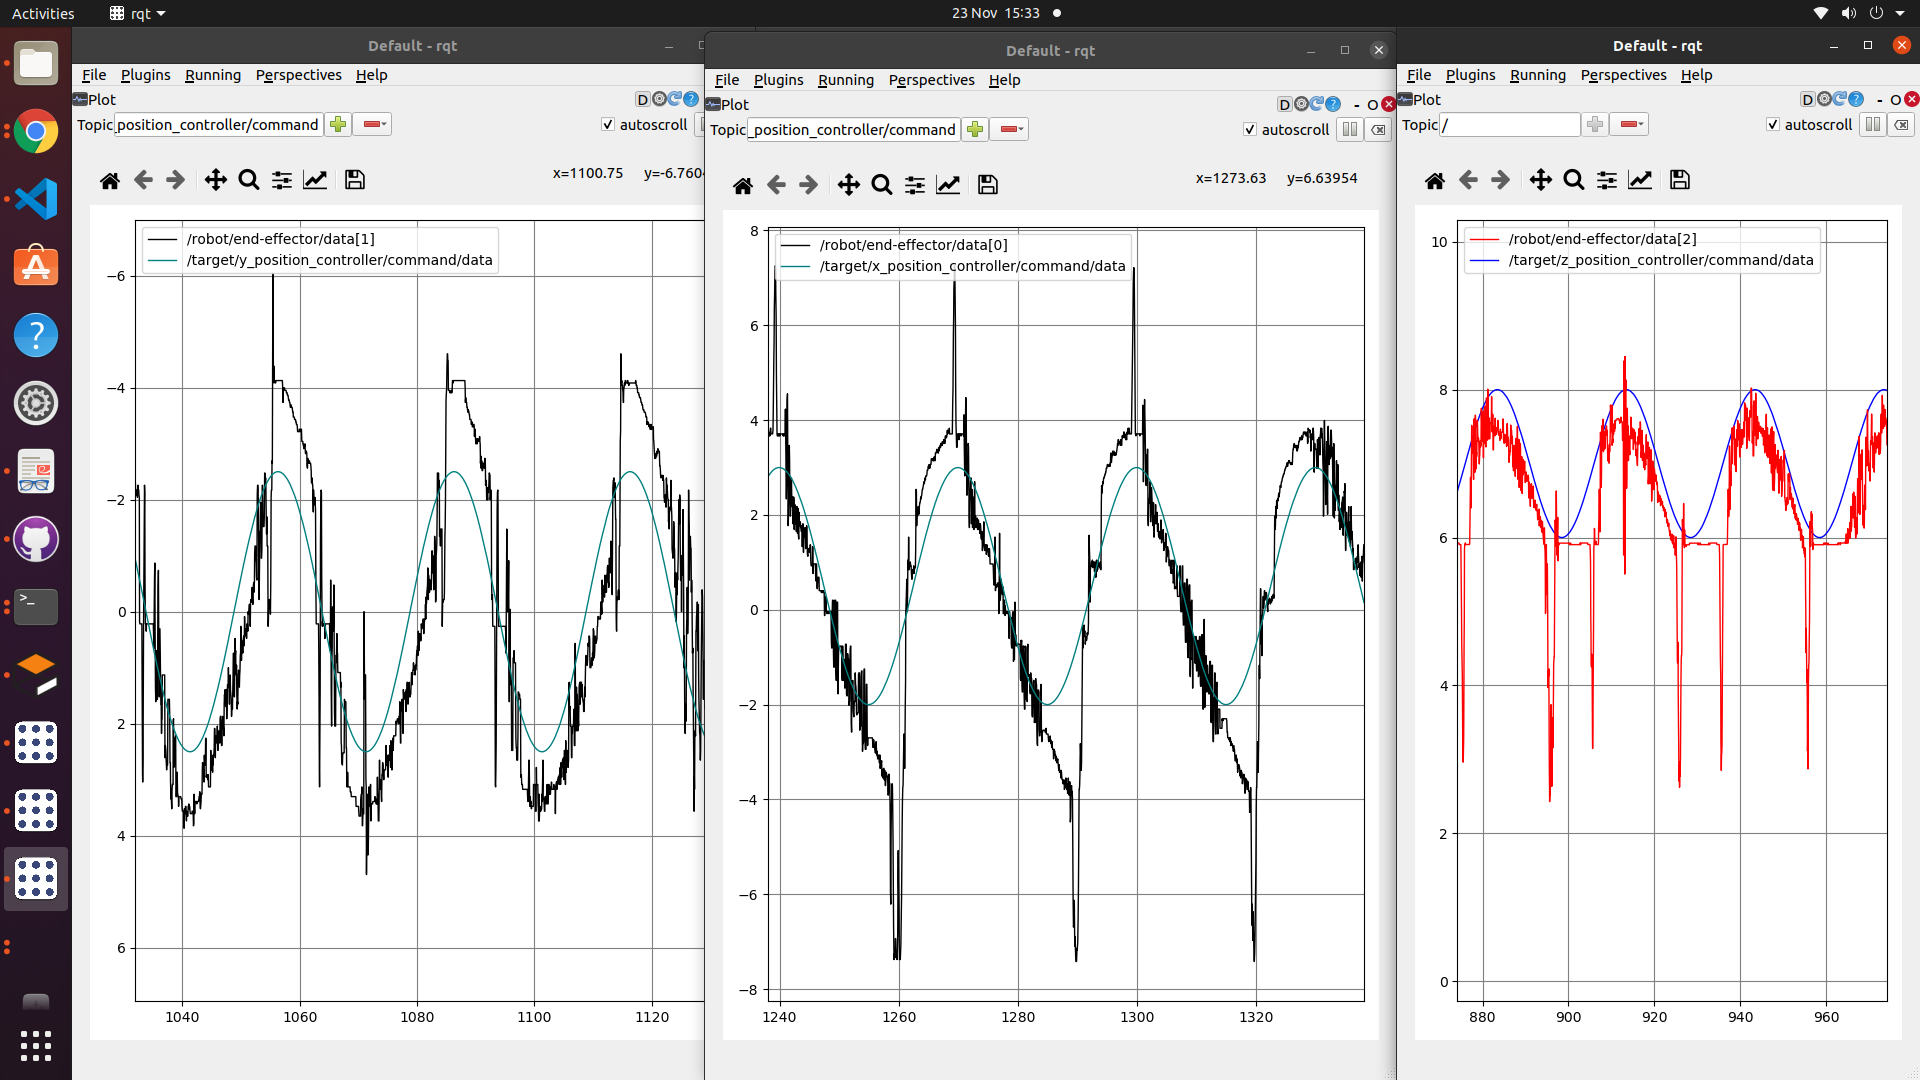
\includegraphics[width=\textwidth]{closed_control_accuracy.png}
\end{landscape}
\end{document}

